% Main report document — Báo cáo về Dữ liệu
% Laptop Price Prediction — CSC14005
% Only preamble, title page, and \input calls

\documentclass[12pt]{article}

%=============================================================================
% REPORT INFORMATION
%=============================================================================
\newcommand{\tenkhoa}{Khoa Công nghệ Thông tin}
\newcommand{\tenmonhoc}{CSC14005 -- Nhập môn học máy}
\newcommand{\tendetaibaocao}{Báo cáo về Dữ liệu:\\Dự đoán Giá Laptop tại Thị trường Việt Nam}
\newcommand{\danhsachsinhvien}{%
Nguyễn Quang Duy & - 23120245 \\[0.1cm]
Lưu Trọng Hiếu & - 23120258 \\[0.1cm]
Văn Đình Hiếu & - 23120260%
}
\newcommand{\hovatenGV}{TS. Bùi Tiến Lên}
\newcommand{\thangnam}{Tháng 5, 2026}
%=============================================================================

%----------------------------------------------------------------------------------------
% PACKAGES
%----------------------------------------------------------------------------------------
\usepackage[T5]{fontenc}
\usepackage[utf8]{inputenc}
\usepackage[english,vietnamese]{babel}
\usepackage{amsmath, amssymb}
\usepackage{graphicx}
\usepackage[colorinlistoftodos]{todonotes}
\usepackage{listings}
\usepackage{booktabs}
\usepackage{float}
\usepackage{geometry}
\usepackage{fancyhdr}
\usepackage{lastpage}
\usepackage{xcolor}
\usepackage{subcaption}
\usepackage{enumitem}
\usepackage{tikz}
\usepackage{pgfplots}
\pgfplotsset{compat=1.18}
\usepackage{multirow}
\usepackage{colortbl}
\usepackage{tcolorbox}
\usepackage{tabularx}
\usepackage{array}
\usepackage{microtype}
\usepackage{csquotes}
\usepackage{longtable}

\setlength{\marginparwidth}{2cm}

\usepackage[unicode,bookmarksnumbered,bookmarksopen]{hyperref}

\geometry{a4paper, margin=2.5cm, top=3.5cm, bottom=2.5cm, headheight=1.6cm, headsep=0.8cm}

\hypersetup{
    unicode=true,
    pdfencoding=unicode,
    colorlinks=true,
    linkcolor=blue,
    filecolor=magenta,
    urlcolor=cyan,
    citecolor=blue,
}

% Superscript citation style
\let\oldcite\cite
\renewcommand{\cite}[1]{\textsuperscript{\oldcite{#1}}}

\usepackage[nameinlink]{cleveref}
\crefname{figure}{Hình}{Hình}
\crefname{table}{Bảng}{Bảng}
\crefname{section}{Mục}{Mục}

% Code listing style
\lstset{
    basicstyle=\ttfamily\small,
    breaklines=true,
    frame=single,
    numbers=left,
    numberstyle=\tiny,
    language=Python,
    backgroundcolor=\color{gray!10},
    keywordstyle=\color{blue},
    commentstyle=\color{green!60!black},
    stringstyle=\color{orange},
    showstringspaces=false
}

\graphicspath{{images/}{logo/}}

%----------------------------------------------------------------------------------------
% HEADER AND FOOTER
%----------------------------------------------------------------------------------------
\pagestyle{fancy}
\fancyhf{}

\fancyhead[L]{%
    \raisebox{0.1cm}{
\includegraphics[height=0.7cm]{logo/logo_khtn.png}}%
    \hspace{0.3cm}%
    \begin{tabular}[b]{@{}l@{}}
        {\footnotesize\textbf{Trường đại học Khoa Học Tự Nhiên TP.HCM}} \\
        {\scriptsize \tenkhoa}
    \end{tabular}
}
\fancyhead[C]{}
\fancyhead[R]{}
\fancyfoot[L]{\footnotesize \tenmonhoc}
\fancyfoot[C]{}
\fancyfoot[R]{\footnotesize Trang \thepage/\pageref*{LastPage}}
\renewcommand{\headrulewidth}{0.4pt}
\renewcommand{\footrulewidth}{0.4pt}

\fancypagestyle{plain}{
    \fancyhf{}
    \fancyhead[L]{%
        \raisebox{0.1cm}{
\includegraphics[height=0.7cm]{logo/logo_khtn.png}}%
        \hspace{0.3cm}%
        \begin{tabular}[b]{@{}l@{}}
            {\footnotesize\textbf{Trường đại học Khoa Học Tự Nhiên TP.HCM}} \\
            {\scriptsize \tenkhoa}
        \end{tabular}
    }
    \fancyfoot[L]{\footnotesize \tenmonhoc}
    \fancyfoot[R]{\footnotesize Trang \thepage/\pageref*{LastPage}}
    \renewcommand{\headrulewidth}{0.4pt}
    \renewcommand{\footrulewidth}{0.4pt}
}

%----------------------------------------------------------------------------------------
% DOCUMENT
%----------------------------------------------------------------------------------------
\begin{document}

%--- Title Page ---
\begin{titlepage}
\newcommand{\HRule}{\rule{\linewidth}{0.5mm}}
\center


\includegraphics[width=0.2\textwidth]{logo/rsz_3logo-khtn.png}\\[0.5cm]
\textsc{\LARGE Trường Đại học Khoa Học Tự Nhiên}\\[0.3cm]
\textsc{\LARGE TP. Hồ Chí Minh}\\[1cm]
\textsc{\Large \tenkhoa}\\[0.5cm]
\textsc{\large Môn học: \tenmonhoc}\\[1cm]

\HRule \\[0.4cm]
{\huge \bfseries \tendetaibaocao}\\[0.4cm]
\HRule \\[1.5cm]

\begin{minipage}[t]{0.55\textwidth}
\begin{flushleft} \large
\emph{Nhóm sinh viên thực hiện:}\\
\vspace{0.1cm}
\begin{tabular}{@{}ll@{}}
\danhsachsinhvien
\end{tabular}
\end{flushleft}
\end{minipage}
\hfill
\begin{minipage}[t]{0.4\textwidth}
\begin{flushright} \large
\emph{Giảng viên hướng dẫn:} \\
\vspace{0.1cm}
\hovatenGV
\end{flushright}
\end{minipage}\\[2cm]

{\large \thangnam}\\[2cm]
\vfill
\end{titlepage}

%--- Table of Contents ---
{\hypersetup{linkcolor=black}
\tableofcontents
\newpage
\addcontentsline{toc}{section}{Danh mục hình ảnh}
\listoffigures
\newpage
\addcontentsline{toc}{section}{Danh mục bảng biểu}
\listoftables}

%--- Sections ---
\newpage
\addcontentsline{toc}{section}{Danh mục từ viết tắt}
\section*{Danh mục từ viết tắt}

\noindent
\renewcommand{\arraystretch}{1.5}
\begin{tabularx}{\textwidth}{>{\bfseries}l X}
\toprule
\rowcolor{blue!10}
Từ viết tắt & \textbf{Ý nghĩa} \\
\midrule
EDA   & Exploratory Data Analysis (Phân tích khám phá dữ liệu) \\
IQR   & Interquartile Range (Khoảng tứ phân vị) \\
MNAR  & Missing Not At Random (Dữ liệu thiếu không ngẫu nhiên) \\
API   & Application Programming Interface (Giao diện lập trình ứng dụng) \\
CSV   & Comma-Separated Values (Giá trị phân cách bằng dấu phẩy) \\
SSD   & Solid State Drive (Ổ cứng thể rắn) \\
HDD   & Hard Disk Drive (Ổ đĩa cứng) \\
GPU   & Graphics Processing Unit (Bộ xử lý đồ họa) \\
CPU   & Central Processing Unit (Bộ xử lý trung tâm) \\
RAM   & Random Access Memory (Bộ nhớ truy cập ngẫu nhiên) \\
VND   & Vietnamese Dong (Đồng Việt Nam) \\
MAE   & Mean Absolute Error (Sai số tuyệt đối trung bình) \\
$R^2$ & Coefficient of Determination (Hệ số xác định) \\
\bottomrule
\end{tabularx}


\newpage
\section{Giới thiệu bài toán}
\label{sec:introduction}

Thị trường laptop tại Việt Nam có đặc điểm phân mảnh cao với sự đan xen giữa hai phân khúc chính: laptop mới chính hãng và laptop đã qua sử dụng (second-hand). Giá cả giữa hai phân khúc này chênh lệch đáng kể và chịu ảnh hưởng bởi nhiều yếu tố như cấu hình phần cứng (CPU, RAM, GPU, ổ cứng), thương hiệu, tình trạng máy, chính sách bảo hành, và kích thước màn hình. Việc định giá chính xác một chiếc laptop --- đặc biệt trên các nền tảng thương mại điện tử nơi người bán tự khai báo thông tin --- là một bài toán phức tạp do dữ liệu thường không đồng nhất và chứa nhiều nhiễu.

Báo cáo này trình bày quá trình xây dựng hệ thống dự đoán giá laptop dựa trên phương pháp học máy (Machine Learning). Dữ liệu được thu thập từ hai nguồn trực tuyến: \textbf{Chợ Tốt} --- marketplace cho laptop đã qua sử dụng với 5.866 tin đăng, và \textbf{Websosanh} --- nền tảng so sánh giá cho laptop mới với 4.384 sản phẩm. Hai nguồn dữ liệu bổ sung cho nhau về phạm vi bao phủ thị trường, tuy nhiên đặt ra thách thức về tích hợp do khác biệt về schema, chất lượng dữ liệu, và ngữ nghĩa các trường.

Mục tiêu cụ thể của báo cáo gồm: (1)~mô tả phương pháp và quy trình thu thập dữ liệu từ hai nguồn, (2)~trình bày các bước làm sạch và tiền xử lý, (3)~phân tích khám phá dữ liệu toàn diện với thống kê mô tả và phân tích mối quan hệ giữa các thuộc tính, (4)~đánh giá chất lượng dữ liệu, và (5)~xây dựng baseline model để kiểm chứng khả năng dự đoán giá từ tập dữ liệu đã chuẩn bị.

Cấu trúc báo cáo như sau: \cref{sec:data-collection} trình bày nguồn và phương pháp thu thập dữ liệu. \cref{sec:data-cleaning} mô tả quy trình làm sạch. \cref{sec:data-quality} đánh giá chất lượng dữ liệu. \cref{sec:data-management} nêu cách tổ chức lưu trữ. \cref{sec:eda} là phần phân tích khám phá dữ liệu. \cref{sec:results} trình bày kết quả baseline model. Cuối cùng, \cref{sec:conclusion} tổng hợp các phát hiện chính và định hướng tiếp theo.


\newpage
\section{Phương pháp và nguồn thu thập dữ liệu}
\label{sec:data-collection}

\subsection{Tổng quan nguồn dữ liệu}

Dữ liệu được thu thập từ hai nguồn trực tuyến phổ biến tại Việt Nam, mỗi nguồn đại diện cho một phân khúc thị trường khác nhau. \cref{tab:data-sources} tóm tắt đặc điểm của hai nguồn.

\begin{table}[H]
    \centering
    \caption{So sánh hai nguồn dữ liệu}
    \label{tab:data-sources}
    \begin{tabular}{lcc}
        \toprule
        \textbf{Đặc điểm} & \textbf{Chợ Tốt} & \textbf{Websosanh} \\
        \midrule
        Loại sản phẩm     & Second-hand       & Laptop mới \\
        Số lượng bản ghi   & 5.866             & 4.384 \\
        Số cột             & 15                & 15 \\
        Phương pháp        & Web scraping (HTML) & API + HTML parsing \\
        Đặc điểm dữ liệu  & User-generated, noisy & Structured catalog \\
        Nguồn giá          & Giá đăng bán      & 3 shop price slots \\
        \bottomrule
    \end{tabular}
\end{table}

\subsection{Nguồn 1: Chợ Tốt}
\label{subsec:chotot-collection}

\textbf{Chợ Tốt} (\texttt{chotot.com}) là nền tảng marketplace cho phép người dùng đăng tin bán laptop đã qua sử dụng. Dữ liệu được thu thập qua web scraping\cite{mitchell2018scraping} sử dụng thư viện \texttt{requests}\cite{reitz2011requests} và \texttt{BeautifulSoup}\cite{richardson2007bs4}.

\subsubsection{Quy trình thu thập}

Quy trình gồm hai giai đoạn:

\begin{enumerate}[noitemsep]
    \item \textbf{Trích xuất URL}: Duyệt 300 trang danh mục (category \texttt{cg=8020}), mỗi trang chứa 20 tin đăng. Các URL sản phẩm được trích xuất từ thẻ \texttt{<a>} có class \texttt{cwv3xk0}.
    \item \textbf{Trích xuất chi tiết}: Với mỗi URL, truy cập trang sản phẩm và parse thông tin từ DOM (thẻ \texttt{<div class="p74axq8">} chứa các cặp nhãn--giá trị). Nếu DOM không trả về đủ dữ liệu, fallback sang JSON embedded trong thẻ \texttt{<script id="\_\_NEXT\_DATA\_\_">}.
\end{enumerate}

Mỗi bản ghi gồm: giá, tiêu đề, hãng, dòng máy, tình trạng, chính sách bảo hành, kích cỡ màn hình, bộ vi xử lý, RAM, card màn hình, ổ cứng, loại ổ cứng, xuất xứ, và thông tin sử dụng. Delay giữa các request là 0.1 giây để tránh bị chặn.

\subsubsection{Công cụ sử dụng}

\begin{itemize}[noitemsep]
    \item \texttt{requests} 2.31.0 --- gửi HTTP request
    \item \texttt{beautifulsoup4} 4.14.3 --- parse HTML
    \item Cấu hình lưu tại \texttt{config/chotot\_collection.yml}
\end{itemize}

\subsection{Nguồn 2: Websosanh}
\label{subsec:websosanh-collection}

\textbf{Websosanh} (\texttt{websosanh.vn}) là nền tảng so sánh giá, tổng hợp thông tin laptop mới từ nhiều cửa hàng trực tuyến. Dữ liệu được thu thập qua API kết hợp HTML parsing.

\subsubsection{Quy trình thu thập}

Quy trình gồm ba giai đoạn, được quản lý bởi lớp \texttt{DataCollectionPipeline}:

\begin{enumerate}[noitemsep]
    \item \textbf{Trích xuất URL}: Gửi POST request đến endpoint \texttt{search-api/get-search-product} với payload chứa \texttt{categoryIds=[18]} (laptop). Crawl theo từng brand sử dụng mapping từ \texttt{brand\_mapping.json} (12 hãng: HP, Asus, Lenovo, Acer, Dell, Apple, MSI, Samsung, Sony, Fujitsu, Toshiba, và nhóm ``khác'').
    \item \textbf{Trích xuất thông số}: Với mỗi URL sản phẩm, tải trang HTML và parse bảng \texttt{<table class="table-specifications">} để lấy thông số kỹ thuật.
    \item \textbf{Trích xuất giá}: Gọi API \texttt{compare-api/get-compare-normal-merchant} với \texttt{rootProductId} để lấy giá từ tối đa 3 cửa hàng, gồm tên shop, giá, và link sản phẩm tại shop đó.
\end{enumerate}

Dữ liệu được lưu theo chunk (100 bản ghi/lần) để tránh mất dữ liệu khi gặp lỗi. Delay giữa các request là 0.7 giây.

\subsubsection{Công cụ sử dụng}

\begin{itemize}[noitemsep]
    \item \texttt{requests} 2.31.0 --- gửi HTTP request (GET và POST)
    \item \texttt{beautifulsoup4} 4.14.3 --- parse HTML spec table
    \item \texttt{pandas}\cite{mckinney2010pandas} 2.2.2 --- lưu trữ và xử lý DataFrame
    \item Cấu hình lưu tại \texttt{config/websosanh\_collection.yml}
\end{itemize}

\subsection{Định dạng lưu trữ}

Cả hai nguồn đều lưu trữ dưới dạng CSV:
\begin{itemize}[noitemsep]
    \item \texttt{data/raw/chotot\_laptop\_data.csv} --- 5.866 dòng, 1.54 MB
    \item \texttt{data/raw/laptop\_features.csv} --- raw Websosanh, 3.69 MB
    \item \texttt{data/raw/clean\_laptop\_features.csv} --- Websosanh sau cleaning, 575 KB
\end{itemize}




\newpage
\section{Quy trình làm sạch và tiền xử lý dữ liệu}
\label{sec:data-cleaning}

Dữ liệu thô từ cả hai nguồn chứa nhiều vấn đề cần xử lý trước khi phân tích. Phần này mô tả quy trình làm sạch, được triển khai trong module \texttt{src/data/data\_cleaning.py} và orchestrate bởi \texttt{pipeline/clean\_data\_pipeline.py}.

\subsection{Xử lý chung}

\subsubsection{Loại bỏ ký tự xuống dòng}
Nhiều cột chứa ký tự \texttt{\textbackslash n} do quá trình crawl. Hàm \texttt{clean\_newlines()} thay thế tất cả \texttt{\textbackslash n} bằng dấu phẩy và loại bỏ khoảng trắng thừa cho các cột kiểu \texttt{object}.

\subsubsection{Xử lý trùng lặp}
Kiểm tra trùng lặp được thực hiện theo hai mức: (1)~trùng URL --- không có bản ghi nào trùng URL trong Chợ Tốt, (2)~trùng nội dung (title + price + brand) --- xác nhận không có trùng lặp hoàn toàn. Đối với Websosanh, không có full-row duplicate nhưng tồn tại soft duplicates (cùng cấu hình, khác shop/màu sắc).

\subsection{Xử lý dữ liệu thiếu}

Dữ liệu thiếu phân bố không đồng đều giữa các cột. \cref{tab:missing-chotot} tóm tắt tỷ lệ thiếu của nguồn Chợ Tốt.

\begin{table}[H]
    \centering
    \caption{Tỷ lệ dữ liệu thiếu các cột chính --- Chợ Tốt}
    \label{tab:missing-chotot}
    \begin{tabular}{lrr}
        \toprule
        \textbf{Cột} & \textbf{Số missing} & \textbf{Tỷ lệ (\%)} \\
        \midrule
        Card màn hình       & 1.421 & 24.2 \\
        Kích cỡ màn hình    & 1.056 & 18.0 \\
        Ổ cứng              & 470   & 8.0  \\
        Loại ổ cứng         & 854   & 14.6 \\
        RAM                 & 239   & 4.1  \\
        Bộ vi xử lý         & 237   & 4.0  \\
        Dòng máy            & 0     & 0.0  \\
        Hãng                & 0     & 0.0  \\
        \bottomrule
    \end{tabular}
\end{table}

Phân tích cho thấy missing values tuân theo mô hình \textbf{MNAR} (Missing Not At Random)\cite{rubin1976missing}: các cột spec thường thiếu cùng lúc (tương quan dương), và tỷ lệ thiếu khác nhau theo brand. Nhóm có median giá thấp hơn có xu hướng thiếu nhiều thông tin hơn.

\subsection{Chuẩn hóa và chuyển đổi kiểu dữ liệu}

\subsubsection{Giá (Price)}
\begin{itemize}[noitemsep]
    \item \textbf{Chợ Tốt}: Giá ở dạng chuỗi \texttt{"X.XXX.XXX đ"}, được parse bằng regex loại bỏ ký tự không phải số, chuyển sang numeric.
    \item \textbf{Websosanh}: Ba cột giá (\texttt{shop\_1/2/3\_price}) được chuyển về numeric bằng \texttt{pd.to\_numeric()}. Áp dụng domain filter (loại giá $<$ 3 triệu hoặc $>$ 200 triệu), sau đó tính \texttt{price\_median} từ các giá hợp lệ.
\end{itemize}

\subsubsection{RAM}
Giá trị dạng \texttt{"8 GB"} được loại bỏ ký tự chữ cái và khoảng trắng, chuyển về số nguyên (đơn vị GB). Các giá trị bất thường ($<$ 4 GB hoặc $>$ 128 GB) được kiểm tra và đánh dấu.

\subsubsection{Ổ cứng}
Hàm \texttt{clean\_storage()} xử lý nhiều trường hợp: dung lượng đơn (\texttt{"512GB"}), kết hợp (\texttt{"256GB + 1TB"}), và chuyển đổi đơn vị TB $\rightarrow$ GB (nhân 1024).

\subsubsection{Kích thước màn hình}
Extract giá trị số inch từ chuỗi text bằng regex \texttt{r"\textbackslash d+(\textbackslash.\textbackslash d+)?"}. Đối với Chợ Tốt, giá trị dạng range (\texttt{"13 -- 14.9 inch"}) được map về midpoint.

\subsubsection{CPU}
Phân loại theo ba chiều: \texttt{cpu\_brand} (Intel/AMD/Apple/Qualcomm), \texttt{cpu\_tier} (i3/i5/i7/i9, Ryzen 3/5/7/9), và \texttt{cpu\_gen} (thế hệ). Thông tin được extract từ cả cột structured và title bằng regex.

\subsubsection{GPU}
Hàm \texttt{clean\_gpu()} phân loại GPU thành các nhóm: RTX Series, GTX Series, Intel Iris Xe, Intel UHD Graphics, AMD Radeon, Intel Arc, Apple GPU, và Other GPU dựa trên keyword matching.

\subsubsection{Các cột khác}
Trọng lượng (g $\rightarrow$ kg), tốc độ CPU (GHz), độ phân giải (width $\times$ height), và kích thước vật lý (dài $\times$ rộng $\times$ dày) đều được parse từ text sang giá trị numeric.

\subsection{Kiểm tra nhất quán dữ liệu}

Các cross-check được thực hiện:
\begin{itemize}[noitemsep]
    \item \textbf{Brand vs Title}: $\sim$95\% title chứa đúng brand tương ứng trong cột Hãng.
    \item \textbf{RAM/Storage}: Giá trị extract từ title vs cột structured --- phát hiện $\sim$188 dòng conflict RAM và $\sim$96 dòng conflict storage.
    \item \textbf{Tình trạng vs Title}: $\sim$90 dòng gắn nhãn ``Mới'' nhưng title chứa keyword second-hand (``đẹp 98\%'', ``pin'', ``góp'').
    \item \textbf{Tình trạng vs Bảo hành}: Một số sản phẩm ``Mới'' nhưng ``Hết bảo hành''.
\end{itemize}

\begin{figure}[H]
    \centering
    % FILL-IN: [USER] Thêm biểu đồ missing value heatmap
    % Nguồn: notebook 01a_chotot_inspection.ipynb, cell [25] — msno.heatmap()
    % \includegraphics[width=0.7\textwidth]{images/missing-heatmap.png}
    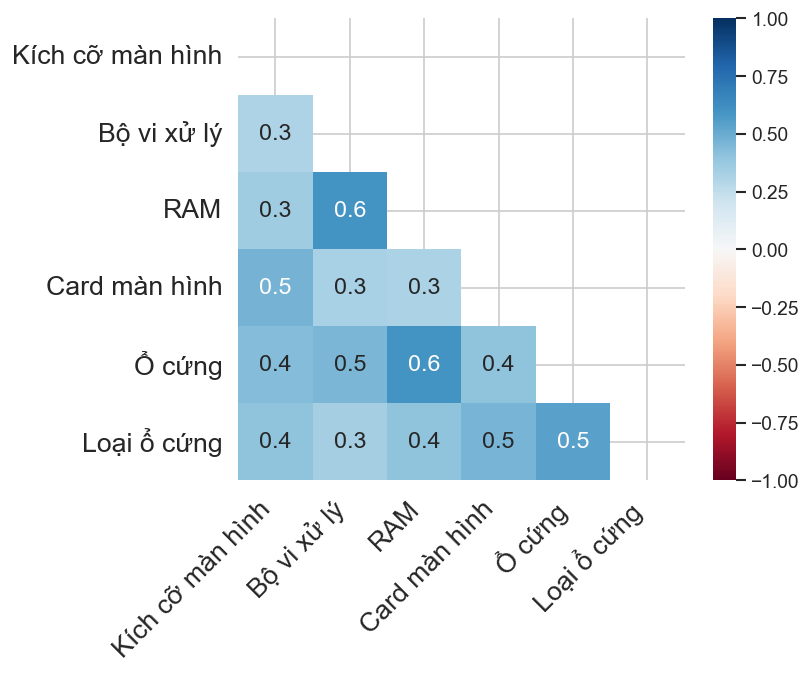
\includegraphics[width=0.7\textwidth]{images/chotot_img_04.png}
    \caption{Heatmap tương quan giữa các cột thiếu dữ liệu trong dataset Chợ Tốt. Giá trị dương (màu sáng) cho thấy các cột spec có xu hướng thiếu cùng lúc, xác nhận mô hình MNAR.}
    \label{fig:missing-heatmap}
\end{figure}


\newpage
\section{Đảm bảo chất lượng dữ liệu}
\label{sec:data-quality}

\subsection{Tổng quan chất lượng}

Sau quá trình thu thập và làm sạch, chất lượng dữ liệu được đánh giá theo bốn tiêu chí: tính đầy đủ (completeness), tính nhất quán (consistency), tính chính xác (accuracy), và tính kịp thời (timeliness).

\begin{table}[H]
    \centering
    \caption{Đánh giá chất lượng dữ liệu theo nguồn}
    \label{tab:data-quality}
    \begin{tabular}{lcc}
        \toprule
        \textbf{Tiêu chí} & \textbf{Chợ Tốt} & \textbf{Websosanh} \\
        \midrule
        Completeness (trung bình) & $\sim$85\% & $\sim$93\% \\
        Consistency (brand--title) & $\sim$95\% & $\sim$98\% \\
        Accuracy (giá hợp lệ) & $>$99\% & $>$95\% (sau lọc outlier) \\
        Timeliness & Q1 2025 & Q1 2025 \\
        \bottomrule
    \end{tabular}
\end{table}

\subsection{Xử lý outlier}

\subsubsection{Outlier giá --- Chợ Tốt}
Giá đăng bán có range từ 100.000 VND đến trên 150 triệu VND. Các giá cực thấp ($<$ 1 triệu) thường là phụ kiện hoặc linh kiện bị gắn nhầm category. Giá cực cao ($>$ 100 triệu) phần lớn hợp lệ (Apple MacBook Pro cấu hình cao). Nhóm nghiên cứu áp dụng domain filter: giữ lại giá trong khoảng 1--150 triệu VND.

\subsubsection{Outlier giá --- Websosanh}
Dữ liệu chứa các giá bất thường (ví dụ 268 triệu, 860 triệu, 1.629 triệu, 2.750 triệu VND) do lỗi crawl hoặc parse. Quy trình lọc gồm hai bước:
\begin{enumerate}[noitemsep]
    \item \textbf{Domain filter}: Null-out giá $<$ 3 triệu hoặc $>$ 200 triệu.
    \item \textbf{Relative filter}: Dùng median giá của từng dòng làm anchor; null-out giá lệch $>$ 2$\times$ hoặc $<$ 0.5$\times$ so với row median.
\end{enumerate}

Sau cleaning, mỗi sản phẩm Websosanh trung bình còn $\sim$2.99 nguồn giá sạch.

\subsubsection{Outlier thuộc tính}
\begin{itemize}[noitemsep]
    \item \textbf{Kích thước màn hình}: Giá trị $>$ 25 inch được null-out (không phù hợp laptop).
    \item \textbf{RAM}: Giá trị 512 hoặc 5.600 GB là lỗi parse (nhầm tốc độ RAM với dung lượng); null-out giá trị $>$ 256 GB.
    \item \textbf{Storage}: Giá trị 6.144 GB ($\approx$ 6TB) kiểm tra thủ công --- một số là cấu hình thật (cộng gộp nhiều ổ).
\end{itemize}

\subsection{Tạo biến phái sinh (Feature Engineering)}

Để giảm phân mảnh (fragmentation) và sparse features, các biến categorical được gom nhóm:

\begin{table}[H]
    \centering
    \caption{Các biến phái sinh chính}
    \label{tab:derived-features}
    \begin{tabular}{lll}
        \toprule
        \textbf{Biến gốc} & \textbf{Biến mới} & \textbf{Nhóm} \\
        \midrule
        Kích thước (inch)  & \texttt{screen\_size\_group} & $<$13, 13--13.9, 14--14.9, 15--15.9, 16--16.9, $\geq$17 \\
        Dung lượng RAM     & \texttt{ram\_tier\_clean}    & $\leq$8GB, 16GB, 32GB, $>$32GB \\
        Dung lượng ổ cứng  & \texttt{storage\_tier\_clean} & $\leq$256GB, 512GB, 1TB, 2TB, $>$2TB \\
        GPU model          & \texttt{gpu\_tier\_v2}       & Intel Integrated, AMD Radeon, GTX, RTX 4000, RTX 5000, Apple, Other \\
        Loại CPU           & \texttt{cpu\_tier}           & Low-end, Mid-range, High-end, Unknown \\
        \bottomrule
    \end{tabular}
\end{table}

\subsection{Chất lượng biến Unknown}

Sau toàn bộ quá trình cleaning, tỷ lệ Unknown còn lại ở Websosanh:
\begin{itemize}[noitemsep]
    \item \texttt{ram\_type\_clean}: 7.44\%
    \item \texttt{cpu\_tier}: 6.93\% (304 dòng)
    \item \texttt{storage\_tier\_clean}: 5.13\%
    \item \texttt{storage\_type\_clean}: 5.06\%
    \item \texttt{gpu\_tier\_v2}: 4.72\% (207 dòng)
    \item \texttt{brand\_clean}: 4.11\%
\end{itemize}

Các nhóm Unknown được giữ lại như một category riêng thay vì xóa dòng, nhằm tránh mất mẫu và bias.


\newpage
\section{Lưu trữ và quản lý dữ liệu}
\label{sec:data-management}

\subsection{Cấu trúc thư mục}

Dự án được tổ chức theo mô hình modular, phân tách rõ giữa mã nguồn, dữ liệu, pipeline, và cấu hình:

\begin{lstlisting}[language={}, basicstyle=\ttfamily\small, frame=single, caption={Cấu trúc thư mục dự án}, label={lst:project-structure}]
Laptop-Price-Prediction/
  config/
    chotot_collection.yml
    websosanh_collection.yml
  data/raw/
    chotot_laptop_data.csv       (5.866 rows, 1.54 MB)
    laptop_features.csv          (raw websosanh, 3.69 MB)
    clean_laptop_features.csv    (cleaned, 575 KB)
    websosanh_product_links.txt  (URLs, 442 KB)
  src/data/
    chotot_collect.py
    collect.py
    data_cleaning.py
  pipeline/
    collection_data_pipeline.py
    clean_data_pipeline.py
  scripts/
    chotot_collection_run.py
    collection_data_run.py
  notebooks/data/
    01a_chotot_inspection.ipynb
    01b_websach_inspection.ipynb
  artifacts/encoders/
    brand_mapping.json
\end{lstlisting}

\subsection{Quản lý cấu hình}

Cấu hình cho mỗi nguồn được lưu dưới dạng YAML, cho phép thay đổi các tham số scraping (base URL, headers, delay, số trang) mà không cần sửa mã nguồn. File \texttt{brand\_mapping.json} chứa ánh xạ 12 hãng laptop $\rightarrow$ ID category của Websosanh.

\subsection{Định dạng lưu trữ}

Toàn bộ dữ liệu sử dụng định dạng CSV (Comma-Separated Values) với encoding UTF-8. CSV được chọn vì: (1)~đơn giản và tương thích cao với \texttt{pandas}\cite{mckinney2010pandas}, (2)~dễ kiểm tra bằng text editor, và (3)~phù hợp với quy mô dữ liệu ($<$ 10 MB tổng cộng). Đối với dự án lớn hơn, có thể xem xét Parquet hoặc database engine, tuy nhiên ở quy mô hiện tại CSV là đủ hiệu quả.

\subsection{Pipeline tái tạo}

Toàn bộ quy trình từ thu thập đến cleaning có thể tái tạo bằng cách chạy lần lượt:
\begin{lstlisting}[language=bash, caption={Lệnh tái tạo dữ liệu}, label={lst:reproduce}]
# 1. Thu thap du lieu
python scripts/chotot_collection_run.py
python scripts/collection_data_run.py --brand all

# 2. Lam sach du lieu
python scripts/data_cleaning.py
\end{lstlisting}

Mỗi script hỗ trợ tham số dòng lệnh (argparse) để kiểm soát phạm vi crawl và các option cleaning.


\newpage
\section{Phân tích khám phá dữ liệu (EDA)}
\label{sec:eda}

Phần này trình bày kết quả phân tích khám phá dữ liệu\cite{tukey1977eda} trên cả hai nguồn. Các phân tích bao gồm thống kê mô tả, phân phối biến mục tiêu, phân tích đơn biến (univariate) và đa biến (multivariate), cùng kiểm tra tương quan giữa các thuộc tính.

\subsection{Thống kê mô tả tổng quan}

\cref{tab:descriptive-chotot} tóm tắt thống kê mô tả các biến numeric chính của Chợ Tốt.

\begin{table}[H]
    \centering
    \caption{Thống kê mô tả --- Chợ Tốt (biến numeric sau cleaning)}
    \label{tab:descriptive-chotot}
    \begin{tabular}{lrrrrr}
        \toprule
        \textbf{Biến} & \textbf{N} & \textbf{Mean} & \textbf{Median} & \textbf{IQR} & \textbf{Missing (\%)} \\
        \midrule
        price (triệu VND)     & 5.865 & 12.5 & 8.0 & 5.0--15.0 & 0.02 \\
        RAM (GB)               & 5.627 & 10.1 & 8.0 & 8--16 & 4.1 \\
        Storage (GB)           & 5.396 & 373  & 256 & 256--512 & 8.0 \\
        Kích cỡ màn hình (inch) & 4.810 & 14.5 & 14.0 & 13--15.6 & 18.0 \\
        \bottomrule
    \end{tabular}
\end{table}

\begin{table}[H]
    \centering
    \caption{Thống kê mô tả --- Websosanh (biến numeric sau cleaning)}
    \label{tab:descriptive-websach}
    \begin{tabular}{lrrrrr}
        \toprule
        \textbf{Biến} & \textbf{N} & \textbf{Mean} & \textbf{Median} & \textbf{IQR} & \textbf{Missing (\%)} \\
        \midrule
        price\_median (triệu VND) & 4.384 & 23.6 & 18.0 & 12.5--29.0 & 0 \\
        RAM (GB)                   & 4.361 & 14.2 & 16.0 & 8--16 & 0.5 \\
        Storage (GB)               & 4.159 & 584  & 512 & 512--1024 & 5.1 \\
        Kích thước (inch)          & 4.288 & 14.8 & 15.3 & 14--15.6 & 2.2 \\
        \bottomrule
    \end{tabular}
\end{table}

Sự chênh lệch median giá giữa hai nguồn (8 triệu vs 18 triệu) phản ánh đúng bản chất: Chợ Tốt là laptop second-hand, Websosanh là laptop mới.

\subsection{Phân phối biến mục tiêu (Label Distribution)}
\label{subsec:label-distribution}

\subsubsection{Chợ Tốt}
Giá đăng bán có phân phối lệch phải (right-skewed) với mean $\approx$ 12.5 triệu và median $\approx$ 8 triệu VND. Nhóm giá dưới 15 triệu chiếm đa số; nhóm high-end ($>$ 50 triệu) chỉ chiếm $\sim$3\% nhưng kéo đuôi phải đáng kể.

\begin{figure}[H]
    \centering
    % FILL-IN: [USER] Thêm biểu đồ phân phối giá Chợ Tốt
    % Nguồn: notebook 01a, cell [33] — histogram + KDE + boxplot giá
    % \includegraphics[width=0.8\textwidth]{images/price-dist-chotot.png}
    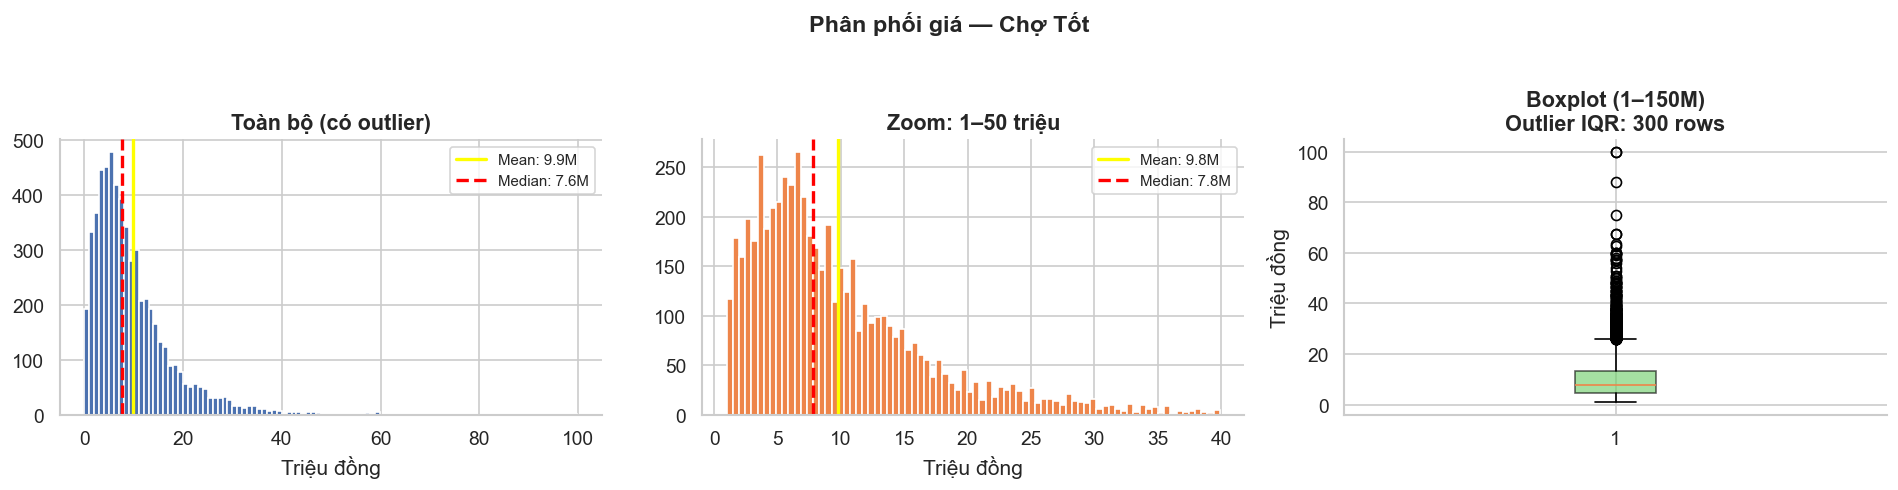
\includegraphics[width=0.8\textwidth]{images/chotot_img_06.png}
    \caption{Phân phối giá laptop trên Chợ Tốt. Histogram (trái) và boxplot (phải) cho thấy dữ liệu lệch phải rõ rệt, với median thấp hơn mean --- đặc trưng của right-skewed distribution.}
    \label{fig:price-dist-chotot}
\end{figure}

\subsubsection{Websosanh}
Biến \texttt{price\_median} (tính từ median 3 nguồn giá) cũng lệch phải nhưng ít hơn so với Chợ Tốt. Skewness $\approx$ 2.65, range từ 3 triệu đến 179.4 triệu VND. Log-transform giúp chuẩn hóa phân phối đáng kể.

\begin{figure}[H]
    \centering
    % FILL-IN: [USER] Thêm biểu đồ phân phối giá Websosanh (gốc vs log)
    % Nguồn: notebook 01b — histogram price_median vs log_price_median
    % \includegraphics[width=0.8\textwidth]{images/price-dist-websach.png}
    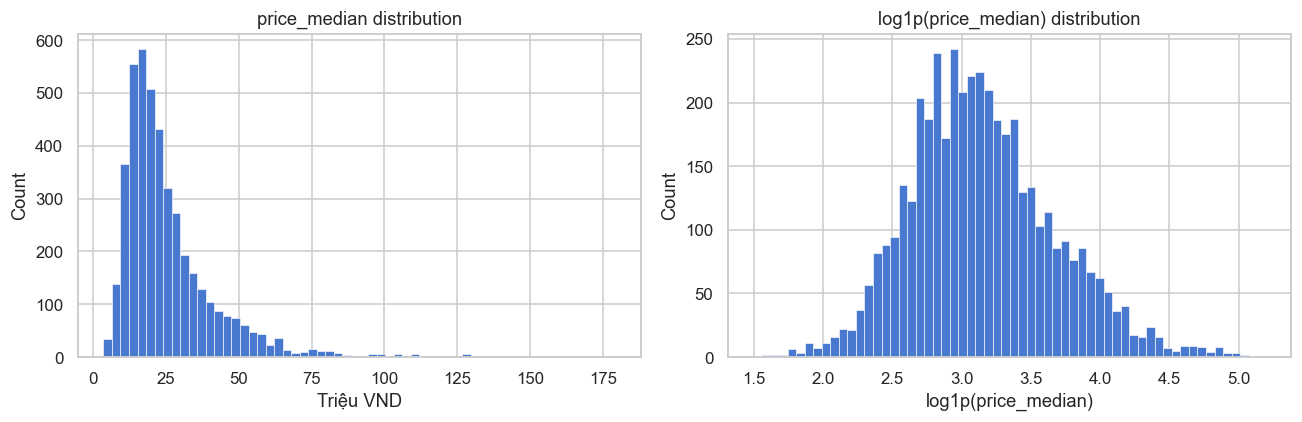
\includegraphics[width=0.8\textwidth]{images/websach_img_20.png}
    \caption{Phân phối giá Websosanh trước và sau log-transform. Log-transform giảm skewness, giúp phân phối gần chuẩn hơn.}
    \label{fig:price-dist-websach}
\end{figure}

\subsection{Phân tích đơn biến}
\label{subsec:univariate}

\subsubsection{Phân phối Brand}

Cả hai nguồn đều cho thấy sự tập trung vào 5 hãng chính: Dell, HP, Asus, Lenovo, và Apple. Trên Chợ Tốt, 5 hãng này chiếm $\sim$80\% listing. Các hãng hiếm ($<$ 30 listing) bao gồm Sony, Fujitsu, Toshiba được cân nhắc gom vào nhóm ``Khác'' khi modeling.

\begin{figure}[H]
    \centering
    % FILL-IN: [USER] Thêm biểu đồ phân phối brand
    % Nguồn: notebook 01a, cell [76] — bar chart brand distribution
    % \includegraphics[width=0.7\textwidth]{images/brand-distribution.png}
    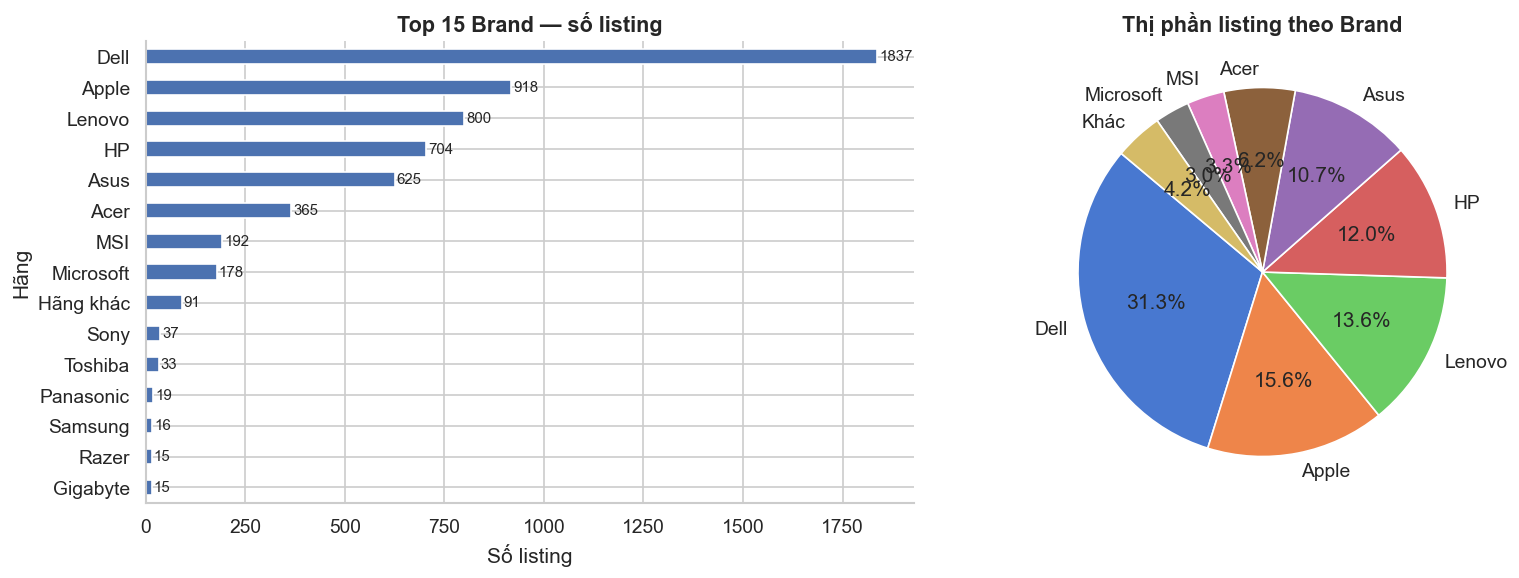
\includegraphics[width=0.7\textwidth]{images/chotot_img_14.png}
    \caption{Phân phối số lượng listing theo brand trên Chợ Tốt. Dell và HP dẫn đầu, theo sau là Asus, Lenovo và Apple.}
    \label{fig:brand-distribution}
\end{figure}

\subsubsection{CPU Brand và CPU Tier}

Intel chiếm $\sim$79.5\% (Chợ Tốt) và $\sim$80.8\% (Websosanh). AMD chiếm 13--15\%, Apple $\sim$3\%, Qualcomm và Microsoft SQ dưới 1\%.

Phân loại CPU tier cho thấy tín hiệu giá rõ: median giá tăng theo thứ tự i3/Ryzen 3 $<$ i5/Ryzen 5 $<$ i7/Ryzen 7 $<$ i9/Ryzen 9. Tuy nhiên CPU tier có confounding với RAM, GPU, và brand (laptop high-end thường có CPU, RAM, GPU đều cao).

\begin{figure}[H]
    \centering
    % FILL-IN: [USER] Thêm biểu đồ CPU distribution + price by CPU tier
    % Nguồn: notebook 01a, cell [170] — subplots CPU brand + CPU tier
    % \includegraphics[width=0.85\textwidth]{images/cpu-analysis.png}
    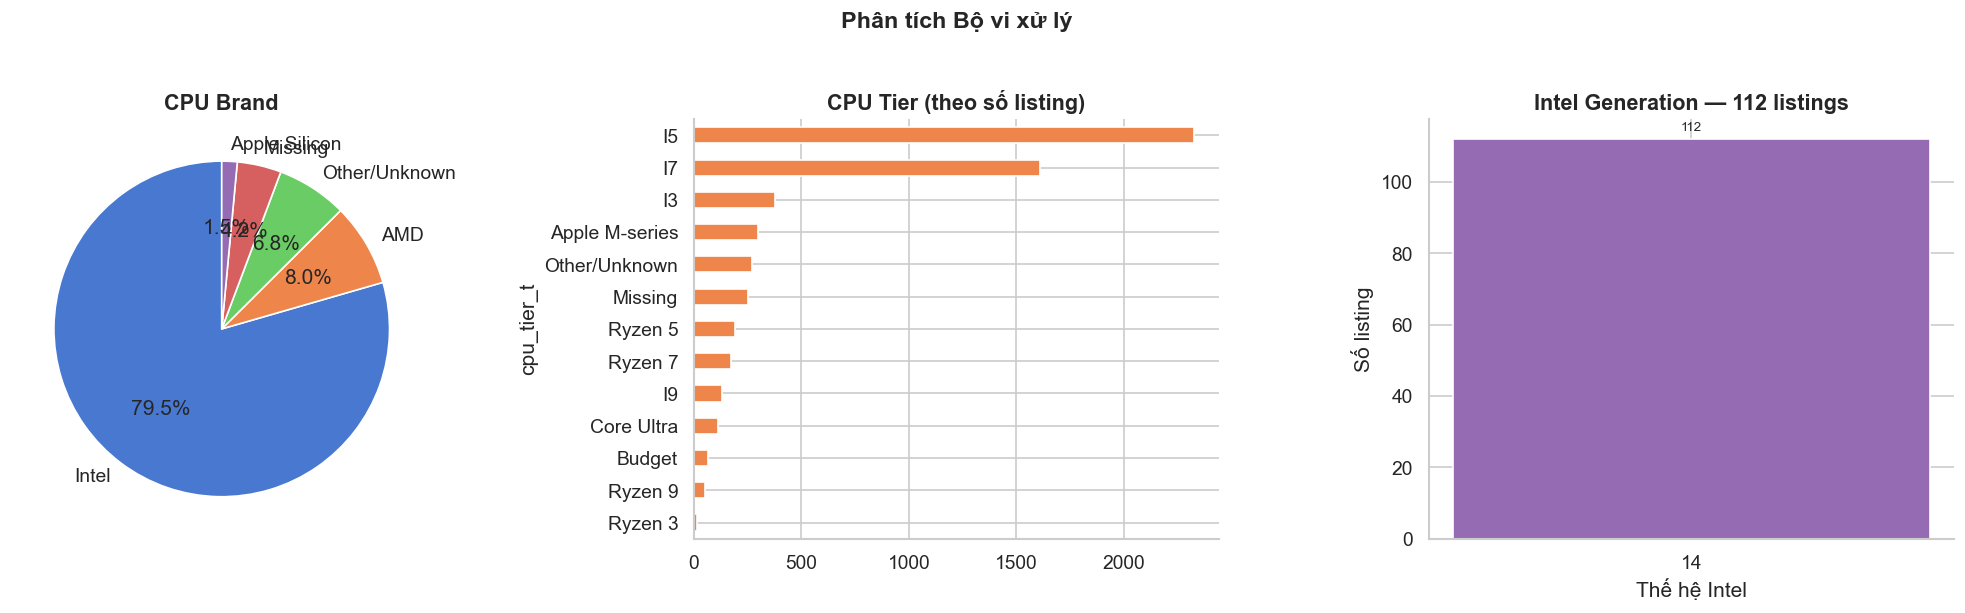
\includegraphics[width=0.85\textwidth]{images/chotot_img_27.png}
    \caption{Phân phối CPU brand (trái) và phân phối giá theo CPU tier (phải). Intel chiếm đa số, giá tăng rõ theo tier.}
    \label{fig:cpu-analysis}
\end{figure}

\subsubsection{RAM}

Hai mức RAM phổ biến nhất là 8GB ($\sim$43\%) và 16GB ($\sim$39\%), cùng chiếm 82.2\% dữ liệu Chợ Tốt. Giá tăng rõ rệt từ 4GB $\rightarrow$ 8GB $\rightarrow$ 16GB $\rightarrow$ 32GB, nhưng mối quan hệ ở các mức hiếm ($<$ 4GB, $>$ 32GB) không ổn định do ít mẫu.

\begin{figure}[H]
    \centering
    % FILL-IN: [USER] Thêm biểu đồ RAM distribution + price by RAM
    % Nguồn: notebook 01a, cell [190] — bar chart + boxplot
    % \includegraphics[width=0.85\textwidth]{images/ram-analysis.png}
    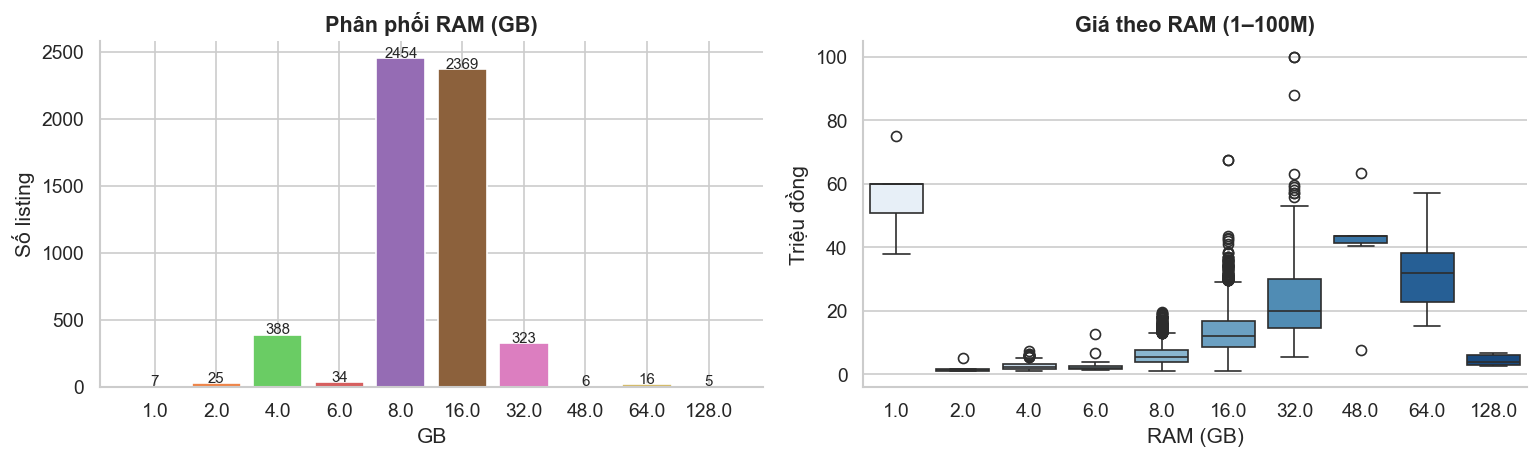
\includegraphics[width=0.85\textwidth]{images/chotot_img_30.png}
    \caption{Phân phối RAM và giá theo mức RAM trên Chợ Tốt. 8GB và 16GB chiếm đa số, giá tăng đơn điệu theo dung lượng ở các mức phổ biến.}
    \label{fig:ram-analysis}
\end{figure}

\subsubsection{GPU}

GPU có tỷ lệ missing cao nhất ($\sim$24\% trên Chợ Tốt, $\sim$4.7\% trên Websosanh). Phân loại GPU tier cho thấy phần lớn là Intel Integrated (UHD/Iris Xe). Nhóm Dedicated GPU (RTX/GTX) có median giá cao hơn đáng kể.

Missing GPU có tính hệ thống theo brand: HP ($\sim$34\% missing) cao hơn Dell ($\sim$19\%).

\subsubsection{Storage}

SSD chiếm ưu thế tuyệt đối ở cả hai nguồn. Dung lượng phổ biến nhất là 256GB và 512GB (Chợ Tốt) hoặc 512GB (Websosanh). Giá tăng theo storage tier: 256GB $<$ 512GB $<$ 1TB $<$ 2TB, tuy nhiên hiệu ứng bị confounding bởi các yếu tố khác.

\subsubsection{Kích thước màn hình}

Nhóm 14--14.9 inch phổ biến nhất ở cả hai nguồn. Giá có xu hướng tăng ở nhóm $\geq$16 inch, nhưng hiệu ứng bị nhiễu bởi cấu hình đi kèm (laptop 16 inch thường là gaming/workstation với GPU rời).

Trên Websosanh, gom kích thước thành 6 nhóm: $<$13, 13--13.9, 14--14.9, 15--15.9, 16--16.9, và $\geq$17 inch.

\subsection{Phân tích đa biến}
\label{subsec:multivariate}

\subsubsection{Giá theo Brand}

Boxplot giá theo top-10 brand cho thấy Apple có median giá cao nhất và IQR rộng nhất. Dell, HP, Lenovo tập trung ở phân khúc trung bình. MSI (gaming) có median cao thứ 2.

\begin{figure}[H]
    \centering
    % FILL-IN: [USER] Thêm boxplot giá theo brand
    % Nguồn: notebook 01a, cell [37] — boxplot price by top-10 brands
    % \includegraphics[width=0.8\textwidth]{images/price-by-brand.png}
    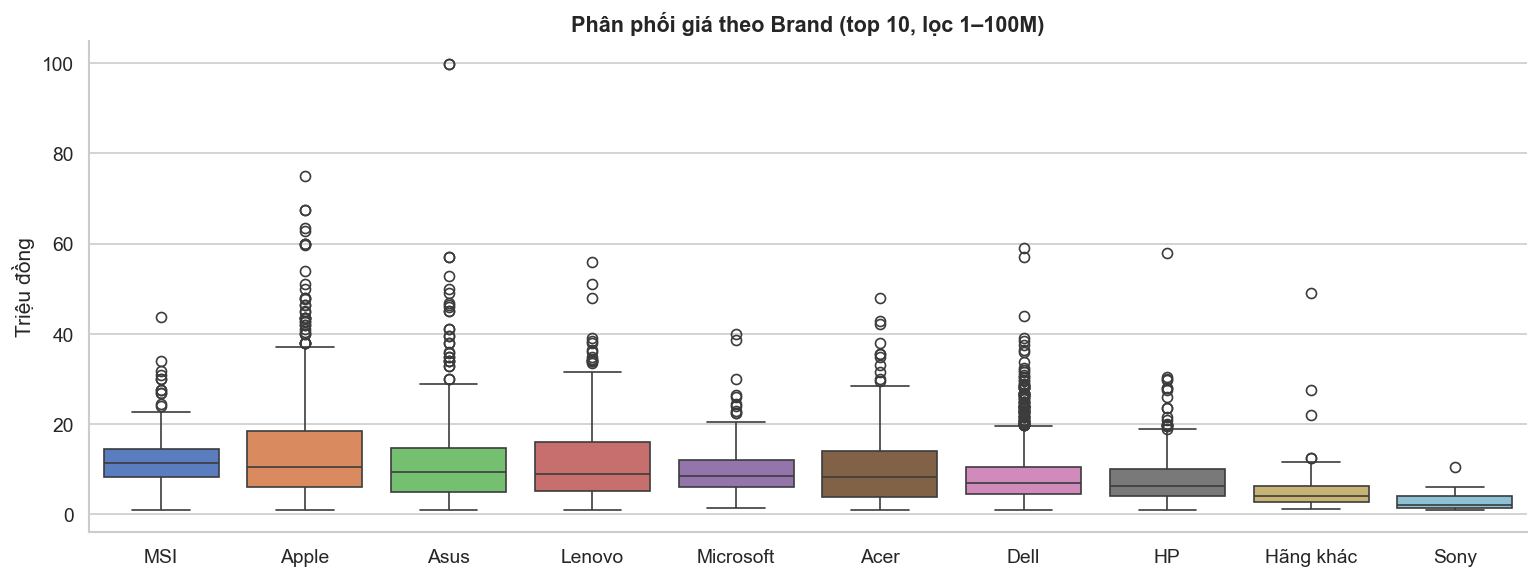
\includegraphics[width=0.8\textwidth]{images/chotot_img_07.png}
    \caption{Phân phối giá theo brand (top 10) trên Chợ Tốt. Apple có median và spread cao nhất, phản ánh định vị premium.}
    \label{fig:price-by-brand}
\end{figure}

\subsubsection{Tương tác giữa các thuộc tính}

Phân tích interaction cho thấy các feature cấu hình không độc lập khi giải thích giá:

\begin{itemize}[noitemsep]
    \item \textbf{CPU $\times$ RAM}: Giá tăng đồng thời theo CPU tier và RAM. Với cùng mức RAM, laptop Intel i7 có giá cao hơn i5; với cùng CPU, RAM 16GB có giá cao hơn 8GB.
    \item \textbf{GPU $\times$ RAM}: Median giá tăng mạnh khi RAM cao kết hợp GPU rời, đặc biệt ở nhóm RTX. Tổ hợp RAM $\geq$16GB + RTX có giá gấp 2--3 lần so với 8GB + Intel Integrated.
    \item \textbf{RAM $\times$ Storage}: Giá tăng rõ khi cả RAM tier và storage tier cùng tăng. Tổ hợp 32GB + 2TB có median price rất cao.
    \item \textbf{Brand $\times$ Screen size}: Cùng nhóm 16--16.9 inch, Apple và MSI có median cao hơn nhiều so với HP hoặc Lenovo.
\end{itemize}

Các tương tác này cho thấy mô hình tuyến tính cần interaction features, hoặc ưu tiên sử dụng tree-based models có thể tự học tương tác phi tuyến\cite{breiman2001random}.

\begin{figure}[H]
    \centering
    % FILL-IN: [USER] Thêm heatmap RAM × Brand × Price
    % Nguồn: notebook 01a, cell [202] — heatmap median price by brand and RAM
    % \includegraphics[width=0.7\textwidth]{images/ram-brand-heatmap.png}
    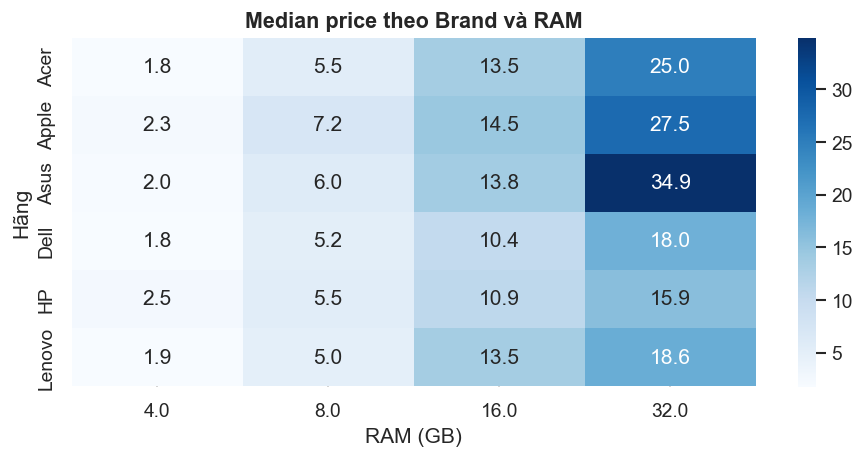
\includegraphics[width=0.7\textwidth]{images/chotot_img_33.png}
    \caption{Heatmap median giá (triệu VND) theo brand và mức RAM trên Chợ Tốt. Giá tăng theo cả hai chiều, với Apple/MSI ở mức cao nhất.}
    \label{fig:ram-brand-heatmap}
\end{figure}

\subsubsection{Tương quan (Correlation)}

Trên Chợ Tốt, RAM có tương quan dương vừa phải với log(price) ($r \approx 0.53$). Storage cũng có tương quan dương nhưng yếu hơn. Tương quan giữa RAM và storage ($r \approx 0.35$) cho thấy multicollinearity ở mức chấp nhận được.

\subsubsection{Phân phối Tình trạng (riêng Chợ Tốt)}

Nhóm ``đã sử dụng chưa sửa'' chiếm $\sim$95\%, gây class imbalance nghiêm trọng. Phát hiện $\sim$90 dòng gắn nhãn ``Mới'' nhưng title chứa keyword second-hand (``đẹp 98\%'', ``pin'', ``góp''), cho thấy label noise.

\subsection{Phân tích dữ liệu phi cấu trúc: Title}
\label{subsec:text-analysis}

Cột \texttt{title} trên Chợ Tốt là text tự do do người dùng nhập. Phân tích cho thấy:
\begin{itemize}[noitemsep]
    \item \textbf{Chất lượng tốt}: 100\% không rỗng, 0\% chỉ chứa khoảng trắng.
    \item \textbf{Brand coverage}: $>$90\% title chứa tên brand, xác nhận tính nhất quán với cột \texttt{Hãng}.
    \item \textbf{Spec keywords}: $\sim$55\% chứa thông tin RAM (pattern ``Xgb'', ``X GB''), $\sim$45\% chứa thông tin storage, $\sim$60\% chứa CPU model.
    \item \textbf{Pattern bán cấu trúc}: 585 title chứa pattern ``X/Y'' (ví dụ ``i5/8GB/256GB''), có thể extract spec từ đây.
    \item \textbf{Rủi ro false positive}: Khi extract RAM bằng regex, giá trị storage (``256GB'', ``512GB'') dễ bị nhầm lẫn. Cần rule loại trừ các giá trị $\geq$ 128 khi parse RAM.
\end{itemize}

\subsection{Dòng máy (Model Line) --- riêng Chợ Tốt}

Cột \texttt{Dòng máy} có 458 giá trị unique, phân phối long-tail cực đoan: 88 dòng máy phổ biến nhất cover 80\% dữ liệu, nhưng 370 dòng còn lại chỉ chiếm 20\%. Khoảng 15\% listing gắn nhãn ``Dòng Khác''. Giá có tín hiệu rõ theo dòng máy (ví dụ MacBook Pro $>$ ThinkPad $>$ Inspiron), nhưng IQR rộng ở hầu hết các dòng.

Để giảm high-cardinality, các dòng có $<$ 10 listing được gom vào ``Other''. Kết hợp Hãng + Dòng máy cho tín hiệu giá mạnh hơn dùng riêng lẻ.


\newpage
\section{Kết quả Baseline Model}
\label{sec:results}

Để đánh giá khả năng dự đoán giá từ dữ liệu đã chuẩn bị, nhóm xây dựng một baseline model trên tập Websosanh (laptop mới, dữ liệu sạch hơn, có 3 nguồn giá).

\subsection{Thiết lập thí nghiệm}

\subsubsection{Target variable}
Biến mục tiêu là \texttt{log\_price\_median} --- log-transform của \texttt{price\_median} nhằm giảm ảnh hưởng của đuôi phải và cải thiện phân phối target (skewness giảm từ $\sim$2.65 về $\sim$0.3 sau log-transform).

\subsubsection{Feature set}
Các biến đầu vào sau feature engineering:
\begin{itemize}[noitemsep]
    \item \textbf{Categorical} (one-hot encoded): \texttt{brand\_clean}, \texttt{cpu\_tier}, \texttt{gpu\_tier\_v2}, \texttt{ram\_tier\_clean}, \texttt{ram\_type\_clean}, \texttt{storage\_type\_clean}, \texttt{storage\_tier\_clean}, \texttt{screen\_size\_group}
    \item \textbf{Numeric} (nếu có): \texttt{ram\_gb\_clean}, \texttt{storage\_gb\_clean}, \texttt{screen\_size\_clean}
\end{itemize}

Missing values ở biến numeric được impute bằng median. Biến categorical giữ nhóm ``Unknown'' thay vì drop dòng.

\subsubsection{Mô hình}
Random Forest Regressor\cite{breiman2001random} từ thư viện \texttt{scikit-learn}\cite{pedregosa2011scikit}, sử dụng cấu hình mặc định (100 cây, không giới hạn max\_depth).

\subsection{Kết quả}

Baseline model đạt các chỉ số trên tập kiểm tra (sanity check):

\begin{table}[H]
    \centering
    \caption{Kết quả baseline Random Forest trên Websosanh}
    \label{tab:baseline-results}
    \begin{tabular}{lc}
        \toprule
        \textbf{Metric} & \textbf{Giá trị} \\
        \midrule
        $R^2$ (log\_price\_median) & 0.746 \\
        MAE (giá gốc, triệu VND) & 5.51 \\
        \bottomrule
    \end{tabular}
\end{table}

Kết quả $R^2 \approx 0.746$ cho thấy các biến cấu hình đã giải thích được khoảng 74.6\% phương sai của log giá. MAE $\approx$ 5.51 triệu VND nghĩa là sai số trung bình khoảng 5.5 triệu cho mỗi dự đoán, tương đương $\sim$30\% so với median giá 18 triệu.

\subsection{Phân tích và hạn chế}

Kết quả baseline cho thấy bộ feature đã chuẩn bị có khả năng dự đoán giá, tuy nhiên cần cải thiện:

\begin{enumerate}[noitemsep]
    \item \textbf{Chưa dùng cross-validation}: Kết quả chỉ là sanity check, cần train/validation/test split hoặc k-fold CV.
    \item \textbf{Chưa tuning hyperparameters}: Mô hình dùng cấu hình mặc định, có thể cải thiện bằng grid search hoặc random search.
    \item \textbf{MAE theo phân khúc giá}: MAE tổng thể $\approx$ 5.5 triệu có thể che giấu lỗi lớn ở nhóm high-end ($>$ 50 triệu). Cần đánh giá MAE/MAPE theo từng price band.
    \item \textbf{Feature importance}: Chưa phân tích feature importance hoặc SHAP values để hiểu đóng góp của từng biến.
    \item \textbf{So sánh mô hình}: Cần so sánh với các mô hình khác (XGBoost\cite{chen2016xgboost}, LightGBM, Linear Regression) để đánh giá tương đối.
    \item \textbf{Nonlinear effects}: Nhiều quan hệ giá--feature là phi tuyến (mô tả ở \cref{subsec:multivariate}), phù hợp với tree-based models.
\end{enumerate}

\begin{figure}[H]
    \centering
    % FILL-IN: [USER] Thêm biểu đồ kết quả baseline (predicted vs actual hoặc residual plot)
    % Nguồn: notebook 01b — baseline model evaluation cells
    % \includegraphics[width=0.7\textwidth]{images/baseline-results.png}
    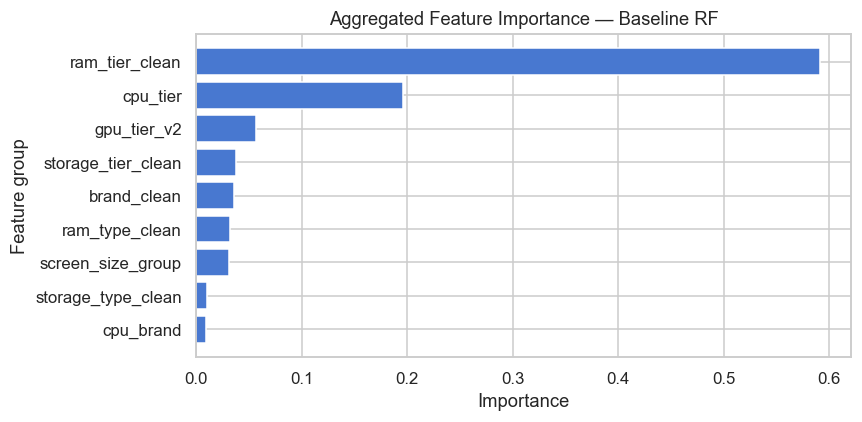
\includegraphics[width=0.7\textwidth]{images/websach_img_21.png}
    \caption{Kết quả dự đoán giá của baseline Random Forest trên Websosanh. Mô hình đạt $R^2 = 0.746$ nhưng có sai số lớn ở nhóm high-end.}
    \label{fig:baseline-results}
\end{figure}


\newpage
\section{Kết luận}
\label{sec:conclusion}

\subsection{Tổng kết}

Báo cáo này trình bày toàn bộ quy trình xây dựng bộ dữ liệu cho bài toán dự đoán giá laptop tại thị trường Việt Nam. Dữ liệu được thu thập từ hai nguồn bổ sung nhau: Chợ Tốt (5.866 listing second-hand) và Websosanh (4.384 sản phẩm mới), mỗi nguồn mang đặc trưng riêng về chất lượng và tính chất dữ liệu.

Các phát hiện chính:

\begin{enumerate}[noitemsep]
    \item \textbf{Chất lượng dữ liệu}: Dữ liệu user-generated (Chợ Tốt) có tỷ lệ missing cao hơn đáng kể so với dữ liệu catalog (Websosanh), đặc biệt ở các cột GPU (24\% vs 4.7\%) và kích thước màn hình (18\% vs 2.2\%). Missing values tuân theo mô hình MNAR --- thiếu có hệ thống theo brand và phân khúc giá.
    \item \textbf{Feature engineering}: Việc gom nhóm các biến categorical (CPU tier, RAM tier, GPU tier, storage tier, screen size group) giúp giảm phân mảnh và tạo tín hiệu giá rõ ràng hơn so với dùng giá trị raw.
    \item \textbf{Confounding}: Các feature cấu hình có tương quan mạnh với nhau (RAM cao $\leftrightarrow$ CPU mạnh $\leftrightarrow$ GPU rời $\leftrightarrow$ brand cao cấp), do đó feature importance cần diễn giải cẩn thận --- không phải quan hệ nhân quả.
    \item \textbf{Baseline model}: Random Forest trên Websosanh đạt $R^2 = 0.746$, MAE $\approx$ 5.51 triệu VND, xác nhận dữ liệu có khả năng dự đoán giá ở mức chấp nhận được.
\end{enumerate}

\subsection{Hạn chế}

\begin{itemize}[noitemsep]
    \item Hai nguồn dữ liệu chưa được tích hợp (merge) thành một tập thống nhất do khác biệt về schema và ngữ nghĩa.
    \item Baseline model chưa qua cross-validation và hyperparameter tuning.
    \item Tỷ lệ Unknown ở một số biến categorical vẫn còn cao ($>$5\%), có thể ảnh hưởng đến hiệu năng model.
    \item Dữ liệu thu thập tại một thời điểm; giá laptop thay đổi nhanh theo thời gian.
\end{itemize}

\subsection{Hướng phát triển}

\begin{enumerate}[noitemsep]
    \item Tích hợp hai nguồn dữ liệu theo schema chung đã thiết kế (\cref{sec:data-collection}).
    \item So sánh nhiều mô hình (XGBoost, LightGBM, CatBoost, Linear Regression) với cross-validation.
    \item Phân tích feature importance và SHAP values để giải thích mô hình.
    \item Đánh giá lỗi dự đoán theo từng phân khúc giá (low, mid, high, premium).
    \item Xây dựng pipeline tự động cập nhật dữ liệu định kỳ.
\end{enumerate}


%--- References ---
\newpage
\bibliographystyle{ieeetr}
\bibliography{references}

\end{document}
